\begin{frame}{Lexical MD Analysis Overview}{cf. \citet{lmdabook}}
\begin{figure}
\centering
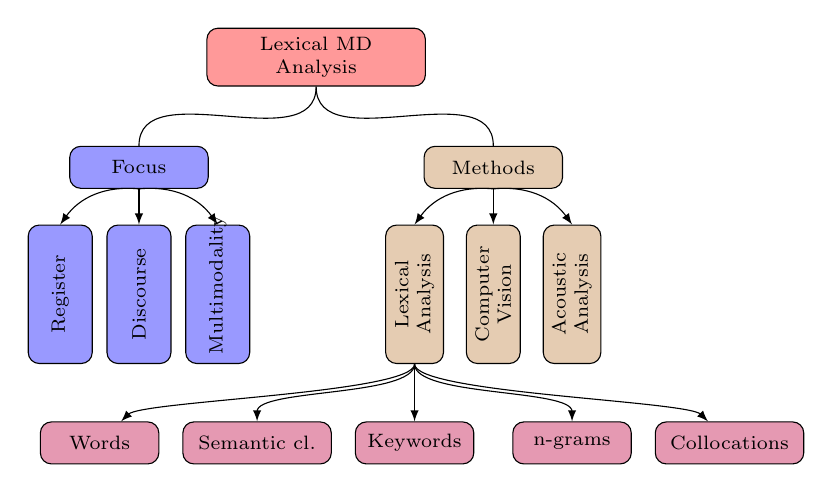
\begin{tikzpicture}

%\tikzstyle{block} = [rectangle, rounded corners, text=black, text centered, draw=black, minimum height=.3in]
\tikzstyle{block} = [rectangle, rounded corners, text=black, anchor=north, text centered, draw=black,font=\scriptsize, minimum height=.21in,  text width=.6in]
\tikzstyle{line} = [-latex,draw=black,line width=.4]
\tikzstyle{noarrow} = [draw=black,line width=.4]

  \node[block,fill=red!40,text=black, text width=1in] (md) at (9.75,9.5) {Lexical MD Analysis};

  \node[block,fill=blue!40,text=black] (focus) at (7.5,8) {Focus};
  \node[block,fill=brown!40,text=black] (methods) at (12,8) {Methods};

  \node[block,fill=blue!40,text=black, rotate=90, anchor=east, minimum height=.32in] (register) at (6.5,7) {Register};
  \node[block,fill=blue!40,text=black, rotate=90, anchor=east, minimum height=.32in] (discourse) at (7.5,7) {Discourse};
  \node[block,fill=blue!40,text=black, rotate=90, anchor=east, minimum height=.32in] (multimodal) at (8.5,7) {Multimodality};

  \node[block,fill=brown!40,text=black, rotate=90, anchor=east] (lexical) at (11,7) {Lexical Analysis};
  \node[block,fill=brown!40,text=black, rotate=90, anchor=east] (computervision) at (12,7) {Computer Vision};
  \node[block,fill=brown!40,text=black, rotate=90, anchor=east] (acoustic) at (13,7) {Acoustic Analysis};

  \node[block,fill=purple!40,text=black, text width=.5in] (words) at (7,4.5) {Words};
  \node[block,fill=purple!40,text=black, text width=.65in, font=\scriptsize] (semantic) at (9,4.5) {Semantic cl.};
  \node[block,fill=purple!40,text=black, text width=.5in, font=\scriptsize] (keywords) at (11,4.5) {Keywords};
  \node[block,fill=purple!40,text=black, text width=.5in, font=\scriptsize] (bundles) at (13,4.5) {n-grams};
  \node[block,fill=purple!40,text=black, text width=.65in, font=\scriptsize] (collocations) at (15,4.5) {Collocations};

%\node[block,fill=green!40,text=black, rotate=90, anchor=east, text width=.5in] (words) at (9,5) {\fontsize{6pt}{10pt}\selectfont Words};

    \draw[noarrow] (md) to[in=90,out=270] (focus); 
    \draw[noarrow] (md) to[in=90,out=270] (methods); 

    \draw[line,-latex] (focus.south) to[bend right] (register.east);
    \draw[line,-latex] (focus.south) to (discourse);
    \draw[line,-latex] (focus.south) to[bend left] (multimodal.east);

    \draw[line,-latex] (methods.south) to[bend right] (lexical.east);
    \draw[line,-latex] (methods.south) to (computervision.east);
    \draw[line,-latex] (methods.south) to[bend left] (acoustic.east);


    \draw[line, looseness=.25] (lexical.west) to[in=45,out=270] (words); 
    \draw[line, looseness=.5] (lexical.west) to[in=90,out=270] (semantic); 
    \draw[line, looseness=.5] (lexical.west) to[in=90,out=270] (keywords); 
    \draw[line, looseness=.5] (lexical.west) to[in=90,out=270] (bundles); 
    \draw[line, looseness=.25] (lexical.west) to[in=135,out=270] (collocations); 

%     \draw[line,-latex] (apply) to[bend right] node[midway,above]{Some label} (languages.east);    
%    \draw[line, densely dashed] (bundapproach) to[in=270,out=90] (bundpattern); 

\end{tikzpicture}
%\caption{MD analysis} 
\label{fig:mdprocedure}
\end{figure}
\end{frame}

